\documentclass{beamer}
\usepackage[french]{babel}
\usepackage{hyperref}
\definecolor{links}{HTML}{2A1B81}
\hypersetup{colorlinks,linkcolor=,urlcolor=links}
\usepackage{graphicx}
\usepackage{amsmath,amssymb}
\usepackage{tabularx}
\usepackage{booktabs}
\usepackage[compatibility=false]{caption}
\usepackage[toc,page]{appendix}
\usepackage{minted}
\usepackage{xspace}

\makeatletter
  \def\beamer@calltheme#1#2#3{%
    \def\beamer@themelist{#2}
    \@for\beamer@themename:=\beamer@themelist\do
    {\usepackage[{#1}]{\beamer@themelocation/#3\beamer@themename}}}

  \def\usefolder#1{
    \def\beamer@themelocation{#1}
  }
  \def\beamer@themelocation{}

\patchcmd{\minted@colorbg}{\noindent}{\medskip\noindent}{}{}
\apptocmd{\endminted@colorbg}{\par\medskip}{}{}
\makeatother

\newcolumntype{Y}{>{\centering\arraybackslash}X}

\usefolder{../theme}
\usetheme[numbering=fraction,block=fill,progressbar=frametitle]{metropolis} %Use metropolis theme

\definecolor{bg}{rgb}{0.95,0.95,0.95}
\setminted{bgcolor=bg,fontsize=\scriptsize,autogobble,mathescape,breaklines,tabsize=2}
\setmintedinline{breaklines,autogobble,fontsize=\scriptsize}
\setbeamersize{text margin left=8pt,text margin right=8pt}
\setbeamercovered{transparent}

\begin{document}

\title[C++]{Introduction à la programmation en C++}
\author[nicolas.audebert@onera.fr]{Nicolas Audebert}
\setmainfont{Fira Sans}


\AtBeginSection[]{
  \begin{frame}{Plan de la séance}
  \small \tableofcontents[currentsection]
  \end{frame}
}

\newcommand\cppi[1]{\mintinline{cpp}{#1}}
\newcommand\cpp[1]{%
  \begin{minted}{cpp}
  #1
  \end{minted}
}%

\subtitle{Les structures}
\date[5 oct. 2018]{Vendredi 5 octobre 2018}
\maketitle

\begin{frame}{Avant toute chose}
  \begin{alertblock}{Rendus de TP et des exercices}
  Les rendus se font sur \href{https://educnet.enpc.fr}{\textbf{Educnet}}.
  \begin{enumerate}
    \item Le code rendu \textbf{doit compiler}.
    \item Le code rendu doit \textbf{être propre} (indentation, noms de variables clairs).
    \item Le code rendu doit \textbf{être commenté} (réponses aux questions, fonctionnement du code).
    \item Rassembler le code dans une seule archive (\texttt{.zip}, \texttt{.rar}, \texttt{.tar.gz}, etc.).
  \end{enumerate}
  \end{alertblock}

\end{frame}

\section{Rappels}


\begin{frame}[fragile=singleslide]
    \frametitle{Propriétés des tableaux statiques}
    Les tableaux statiques sont caractérisés par le \textbf{type} de leurs éléments et leur \textbf{taille}.
	
    \begin{exampleblock}{Exemple}
    \begin{minted}{cpp}
		int mon_tableau[10];
		// Initialisation manuelle à l'aide d'une boucle
		for(int i=0; i < 10; i++){
        	mon_tableau[i] = 5;
		}

		// Déclaration et initialisation directe
		double tableau_reel[5] = {2, 3.2, 9.76, 6, 1000};

		// Déclaration puis initialisation directe
		bool tableau_bool[3];
		tableau_bool = {true, true, false};
    \end{minted}
    \end{exampleblock}
\end{frame}

\begin{frame}[fragile=singleslide]
    \frametitle{Manipulation des tableaux}
    Si \texttt{\textbf{n}} est la taille du tableau, alors les indices vont de \texttt{\textbf{0}} à \texttt{\textbf{n-1}}.
    
    \begin{alertblock}{Attention}
    Tenter d'accéder à un élément hors de ces bornes résultera systématiquement en une erreur lors de l'exécution du programme.
    \end{alertblock}
	
    \begin{exampleblock}{Exemple}
	\begin{minted}{cpp}
const int n = 100; // Taille du tableau (constante)
char tab[n]; // Déclaration du tableau
tab[0] = 'a'; // OK
tab[10] = 'd'; // OK
tab[n-1] = 'k'; // OK
tab[n] = 'f'; // ERREUR
tab[-1] = 'z'; // ERREUR
	\end{minted}
    \end{exampleblock}
\end{frame}

\begin{frame}[fragile=singleslide]
\frametitle{Tableaux et fonctions}

Une fonction peut manipuler un tableau dans sa signature:

\begin{minipage}{0.47\linewidth}
\begin{minted}{cpp}

void affiche(int t[5]){
    for(int i=0; i<5; i++){
    	cout << t[i] << " ";
    }
    cout << endl;
}

\end{minted}
\end{minipage}
\hfill
\begin{minipage}{0.52\linewidth}
\begin{minted}{cpp}

void affiche(int t[], int taille){
    for(int i=0; i<taille; i++){
    	cout << t[i] << " ";
    }
    cout << endl;
}

\end{minted}
\end{minipage}

\begin{alertblock}{Passage par référence}
\begin{itemize}
\item Un tableau est \textbf{toujours} implicitement passé par référence (il ne faut donc pas rajouter de \texttt{\&}).
\item Une fonction \textbf{ne peut pas} retourner de tableau.
\end{itemize}
\end{alertblock}
\end{frame}

\begin{frame}[fragile=singleslide]
\frametitle{Copie et égalité de tableaux}
On ne peut pas copier directement des tableaux entre eux.
\begin{minted}{cpp}
int t1[4] = {1,2,3,4}, t2[4];
t2 = t1 ;
// ERREUR : pas d'affectation avec le = pour les tableaux
\end{minted}

Seule solution : itérer sur les éléments.
\begin{minted}{cpp}
int t1[4] = {1,2,3,4}, t2[4];
for(int i = 0; i < 4; i++){
    t2[i] = t1[i];
}
\end{minted}
De même, pour tester l'égalité entre deux tableaux.
\end{frame}

\begin{frame}[fragile=singleslide]
	\frametitle{Erreurs}
	
	\begin{minted}{cpp}
if(a = 3){...}  // ERREUR: le symbole d'egalite est '=='
if(a == 3){...}
	
for(int i; i < 10; i++){...}  // ERREUR: il faut initialiser i
for(int i = 0; i < 10; i++){...} // OK

if(a && for(int i = 0; i < 100; i++){tab[i]}){...} // ERREUR
		
bool test = true;
for(int i = 0; i < 100; i++){
    if(! tab[i])
        test=false;
}
	\end{minted}
	
\end{frame}

\begin{frame}[fragile=singleslide]
	\frametitle{Erreurs classiques}
	
	\begin{minted}{cpp}
if(a && test){...}
	\end{minted}
		
	\begin{minted}{cpp}
void f(double tab[8]){...} // argument : un tableau

void g(){
    ...
    double vec[8]; // tableau de 8 cases
    f(vec[8]); // ERREUR : vec[nombre] est le contenu d'une case (un nombre)
               // et en plus, la case 8 n'existe pas !
               
    f(vec); // OK on appelle la fonction sur la variable vec (un tableau)
    
}
	\end{minted}
\end{frame}

\section{Pourquoi les structures ?}

\begin{frame}
	\frametitle{Le besoin}
	\begin{block}{Pour l'instant\dots}
		\begin{itemize}
			\item factoriser le code : \textbf{les fonctions}
			\item regrouper les variables de même type : \textbf{les tableaux}
		\end{itemize}
	\end{block}
	\begin{block}{Et maintenant\dots}
		Regrouper des variables qui ne sont pas forcément du même type mais qui forment un ensemble cohérent :
		\begin{itemize}
			\item Contacts : nom, date de naissance, adresse\dots
			\item Dessin : forme, couleur, épaisseur du trait\dots
			\item \dots
		\end{itemize}
	\end{block}
	On utilise des \textbf{structures}.
\end{frame}

\begin{frame}
	\frametitle{Concept}
	{
		\centering
		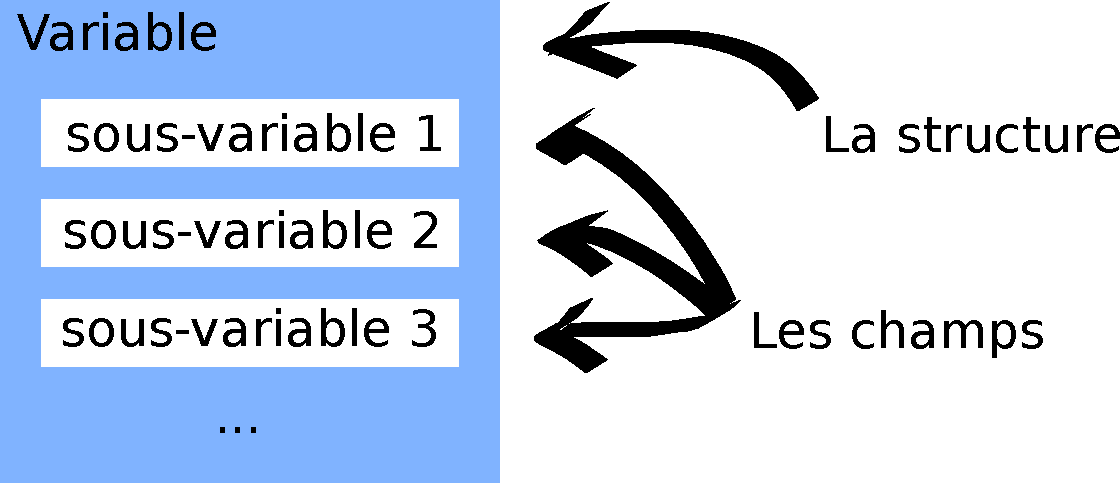
\includegraphics[width=\linewidth]{images/structure.pdf}
	}
	Les structures définissent de nouveaux types.\\
	Les éléments de la structure sont appelés des \textbf{champs}.
\end{frame}

\section{Définition}

\begin{frame}[fragile=singleslide]
	\frametitle{Définir une structure}
	
	\begin{block}{Cas général}
		\begin{minted}{cpp}
struct nom_structure{
	type1 var1; // les champs
	type2 var2;

}; // À ne pas oublier !
        \end{minted}
	\end{block}
	
	La structure définit un nouveau type qui s'utilise comme les autres.
	On accède aux champs avec un \textbf{\huge .}
	
	\begin{block}{Cas général}
	\begin{minted}{cpp}
variable_struct.var1 = 1000;
cout << variable_struct.var2 << endl;
    \end{minted}
	\end{block}
\end{frame}

\begin{frame}
	\frametitle{Structures et tableaux}
	\begin{alertblock}{Tableaux dans les structures}
		Très, très fortement \textbf{DÉCONSEILLÉ} : problèmes liés à l'égalité entre tableaux, notamment dans les retours de fonctions.
	\end{alertblock}
	
	\begin{block}{Tableaux de structures}
		Aucun problème, ils se comportent comme des variables classiques.
	\end{block}
\end{frame}

\begin{frame}[fragile=singleslide]
	\frametitle{Exemple}
	\begin{minipage}{0.47\linewidth}
		\begin{minted}{cpp}
struct Client{
    string nom, prenom;
    string adresse;
    int naissance[3]; // JJ, MM, AAAA
    double taille; 
    double poids;
    bool lunettes;
};




Client cli1;
cli1.nom = "Lovelace"
cli1.prenom = "Ada"
cli1.naissance[0] = 10;
cli1.naissance[1] = 12;
cli1.naissance[2] = 1815;

		\end{minted}
	\end{minipage}
	\hfill
	\begin{minipage}{0.47\linewidth}
		\begin{minted}{cpp}
struct Point{
	double x,y;
};

struct Cercle{
    Point centre;
    double rayon;
    Color couleur;
};

Cercle c;
c.centre.x = 0.5;
c.couleur = RED;
Point pt;
pt.x = pt.y = 5.5;
c.centre = pt;

Point p1={1,2}, p2;
p2 = p1 // OK, recopie champ a champ
		\end{minted}
	\end{minipage}
\end{frame}

\section{Manipulation}

\begin{frame}[fragile=singleslide]
	\frametitle{Initialisation}
	
	\begin{minipage}{0.49\linewidth}
		\begin{minted}{cpp}
Point pt;
pt.x = pt.y = 5.5;

Cercle c;
c.couleur = RED;
c.rayon = 3;
c.centre.x = 5.5;
c.centre.y = 5.5
//ou
c.centre = pt;
		\end{minted}
	\end{minipage}
	\begin{minipage}{0.48\linewidth}
		\begin{minted}{cpp}
Point pt = {5.5};
Cercle c = {pt, 3, RED};

Cercle c={{5.5,5.5},3,RED};
// ERREUR
		\end{minted}
	\end{minipage}
	L'ordre des éléments pour l'initialisation est l'ordre de définition des champs dans la structure.
\end{frame}

\begin{frame}[fragile=singleslide]
	\frametitle{Structures et fonctions}

	Les structures fonctionnent comme des types classiques :
	\begin{minted}{cpp}
// Structure comme argument
void affiche(Point p){
    cout << p.x << " " << p.y << endl;
}

// Structure comme valeur de retour
Point milieu(Point p, Point q){
    Point m;
    m.x = (p.x+q.x)/2;
    m.y = (p.y+q.y)/2;
    return m;
}
	\end{minted}
\end{frame}

\begin{frame}[fragile=singleslide]
	\frametitle{Structures et fonctions}
	
	Les structures fonctionnent comme des types classiques :
		\begin{minted}{cpp}
// Passage par référence
void init(Point &p){
    p.x = 0;
    p.y = 0;
}
		\end{minted}
\end{frame}

\section{TP du jour}

\begin{frame}
	\frametitle{TP : Gravitation}
		\begin{minipage}{0.47\linewidth}
\begin{itemize}
	\item Simulation de système planétaire
	\item Système physique à plusieurs objets
	\item Utilisation des structures
\end{itemize}
\end{minipage}
\hfill
\begin{minipage}{0.47\linewidth}
  \centering
  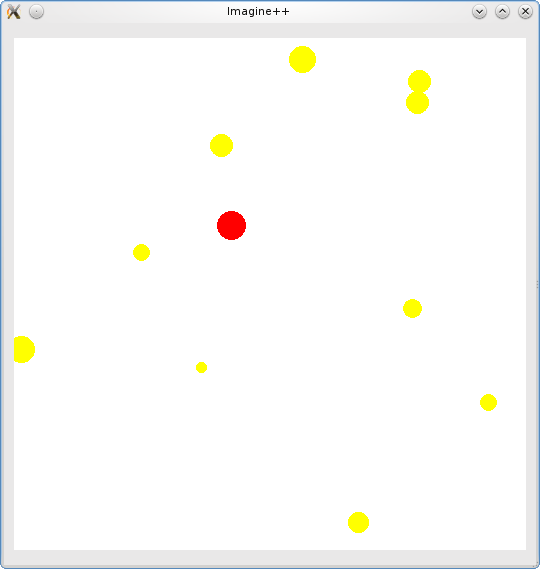
\includegraphics[width=0.9\linewidth]{images/gravit.png}
\end{minipage}
\end{frame}
\end{document}
